%\documentclass[handout]{beamer}
\documentclass{beamer}

% Customize slide appearance
\mode<presentation>
{
  \usetheme{default}
  \setbeamercovered{transparent}
}

\usepackage[english]{babel}
\usepackage{times}
\usepackage{threeparttable}
\usepackage{tabularx}
\usepackage{booktabs}
\usepackage{pgfpages}

\definecolor{darkblue}{rgb}{0.1,0,0.55} \definecolor{darkgreen}{rgb}{0,0.7,0}
\definecolor{important}{rgb}{0.9,0.1,0.1} %
\definecolor{hidden}{rgb}{0.8,0.8,0.8}
\definecolor{darkgreen}{rgb}{0,0.7,0}

%\pgfpagesuselayout{4 on 1}



\AtBeginSection[]
{
  \begin{frame}
  \frametitle{Outline}
  \large{\tableofcontents[currentsection,hideothersubsections]}
  \end{frame}
}


%\usepackage{amstext}

\begin{document}

\begin{frame}

\bigskip

\center{{\Large \textcolor{darkblue}{Seeing is Believing: \\ The Effect of Television on the Identity and Lives of Hispanic People}} \medskip}

\bigskip


\center{\textbf{Andrew Kao} \\ \textit{University of Chicago}}

\bigskip \bigskip

\center{February 2020}

\end{frame}

\begin{frame}
\frametitle{Motivation}


\begin{itemize}
\item Large literature on how TV affects behavior {\footnotesize(Yanigazawa-Drott 2014; DellaVigna \& al. 2007;  Ferrara \&\ al., 2012)}
\item 50\% of Hispanics watch satellite or broadcast Spanish Language TV (SLTV)
\item Complicated time for largest ethnic minority in the US
\item Prior efforts to study Hispanic interaction with media focused on politics {\footnotesize(Waldfogel \& al. 2009; Trujillo \& al. 2012)}
\end{itemize}

This paper examines the effect of SLTV in two ways:\\
\textbf{\,\,\,\, (1) How does Hispanic behavior change in firms and schools?}\\
\textbf{\,\,\,\,  (2) How is identity affected?}

\begin{itemize}
\item Identification: follow Velez \& Newman (2019) and construct spatial RD arising from FCC TV signal regulation
\end{itemize}




\end{frame}


\begin{frame}
\frametitle{Main Findings - Firms}

\centering
        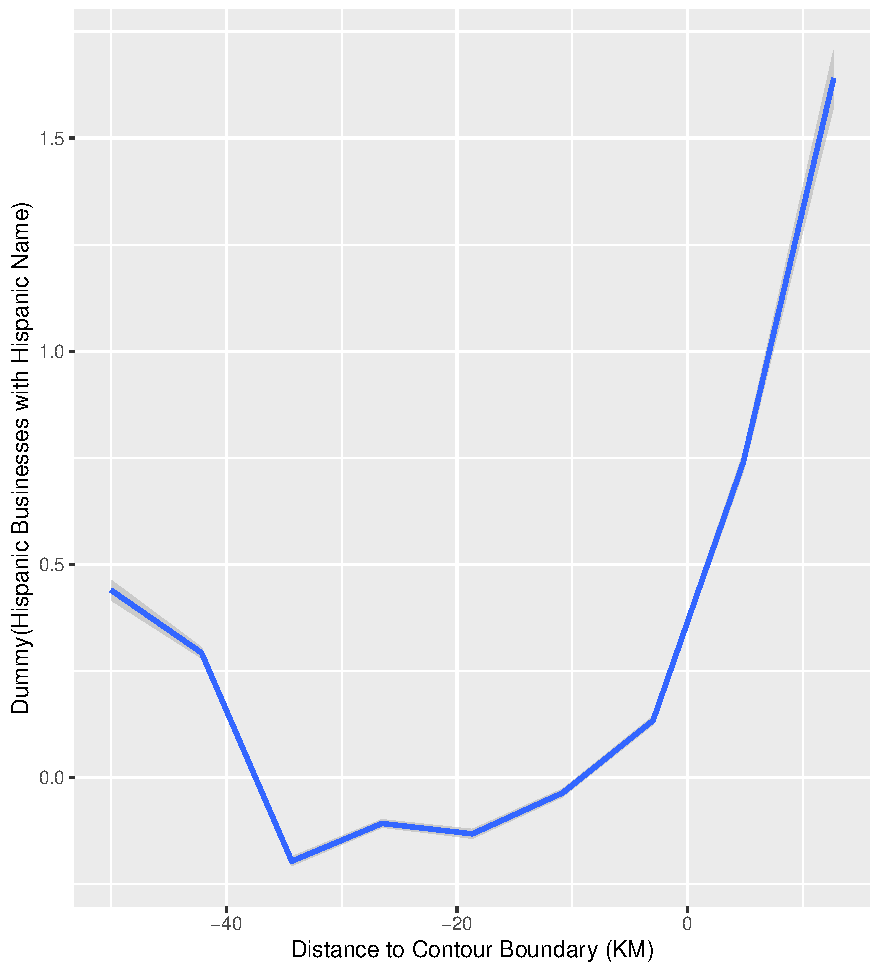
\includegraphics[width=0.65\textwidth]{../../analysis/Output/graphs/hispanicbusnname.pdf}\\
\end{frame}

\begin{frame}
\frametitle{Main Findings - Schools}
\centering
        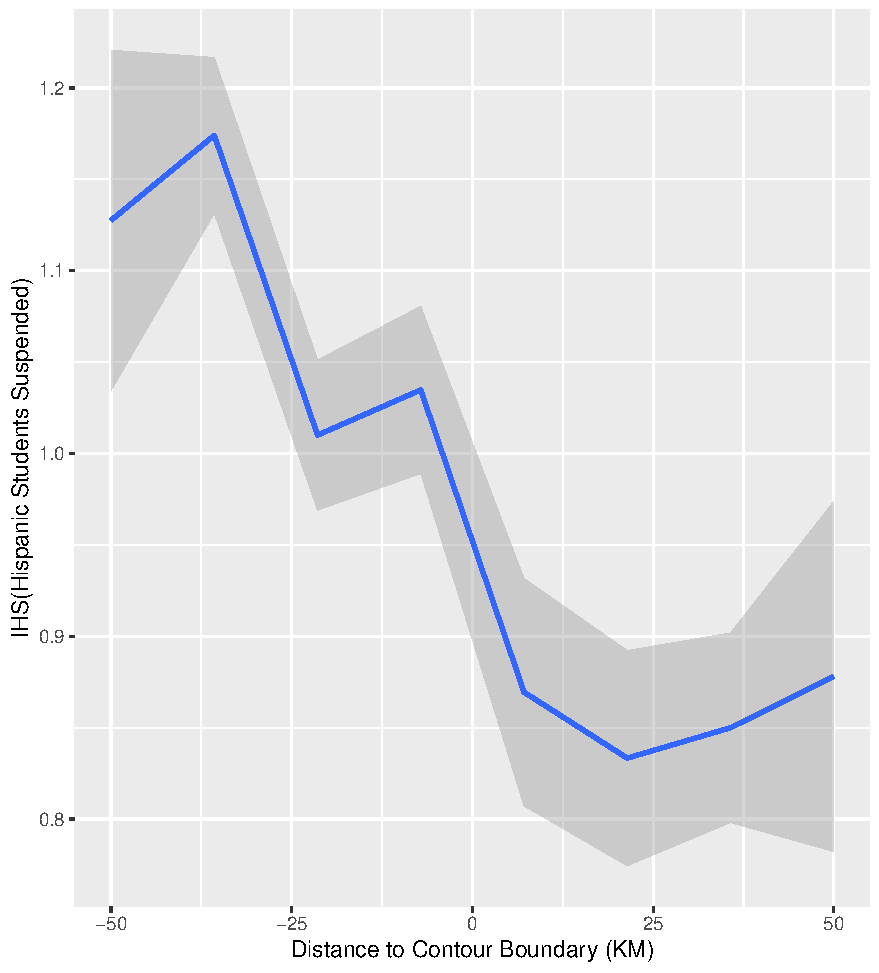
\includegraphics[width=0.65\textwidth]{../../analysis/Output/graphs/hispanicsuspensions.pdf}\\
\end{frame}

\begin{frame}
\frametitle{Main Findings - Campaign Contributions}
\centering
        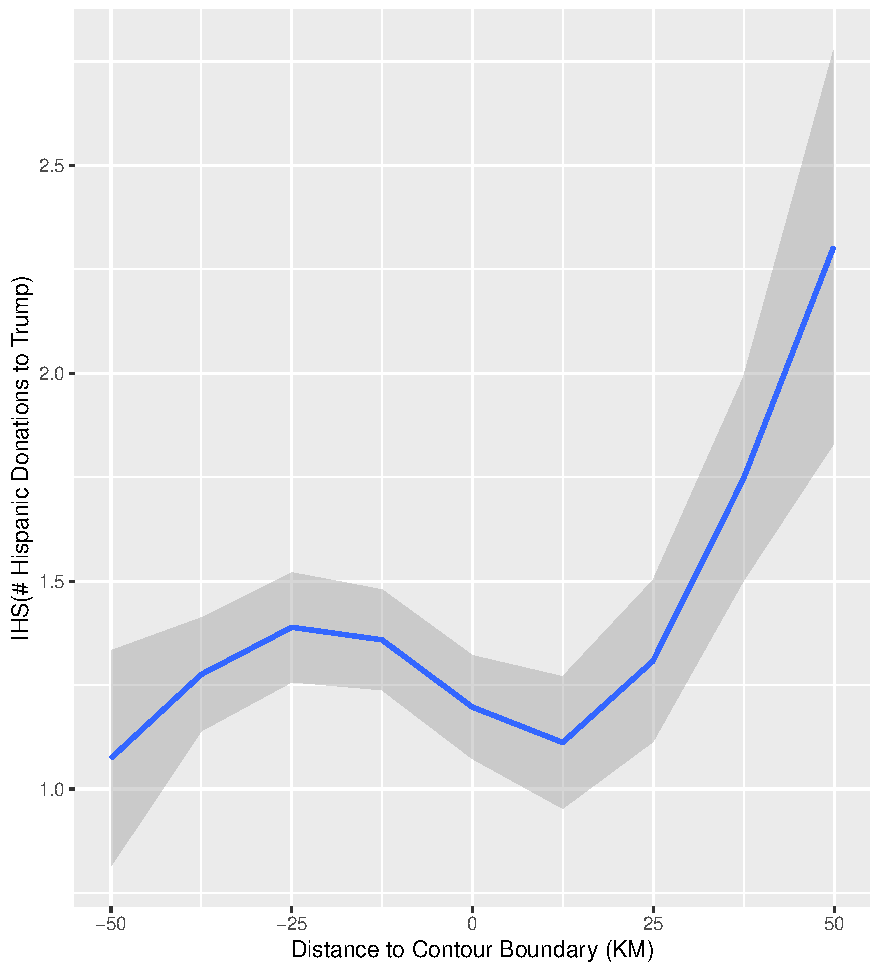
\includegraphics[width=0.65\textwidth]{../../analysis/Output/graphs/hispanictrump.pdf}\\
\end{frame}


\begin{frame}
\frametitle{Contribution}
\begin{itemize}

\item Existing work on Hispanic communities often geographically constrained \& media studies only concerned with effect on politics  {\footnotesize (Velez \& Newman (2019); Trujillo \& al. 2012)}. 
\item[$\rightarrow $] \textcolor{darkblue}{Identify causal effect on larger scale and with more granularity (geocoded microdata)}

\item[$\rightarrow $] \textcolor{darkblue}{Provide a first look at how media affects business and schooling outcomes for Hispanics}

\item Existing research that shows identity is a powerful mechanism {\footnotesize (Benjamin \& al. 2007; Bursztyn \& al. 2015)}. New research on how identity is constructed and strengthened {\footnotesize (Atkin \& al. 2019; Bazzi \& al. 2019)}

\item[$\rightarrow $] \textcolor{darkblue}{Supply a revealed preference demonstration of how identity can be bolstered by the media}

\end{itemize}

\end{frame}


\begin{frame}
\frametitle{Empirical Strategy}
\begin{itemize}

\item OET Bulletin No. 69 --- protect TV stations in (50,90) coverage contour areas
\begin{itemize}
\item Mechanical formula based on geographic/technical factors (not political/economic)
\item Fairly large boundaries that typically cut through small towns/suburbs
\item Purchase/constructed antennas prior to 1977
\end{itemize}
\item Spanish Language TV: Isolate effect on Hispanic communities
\item Both RD and instrument with distance
\begin{itemize}
\item Keep observations within 100 KM of boundary for comparability
\item Focus on the RD, dummy for whether observation falls inside contour
\end{itemize}

\end{itemize}

\end{frame}

\begin{frame}
\frametitle{Coverage Map for TV Station WUVC-DT}
\centering
        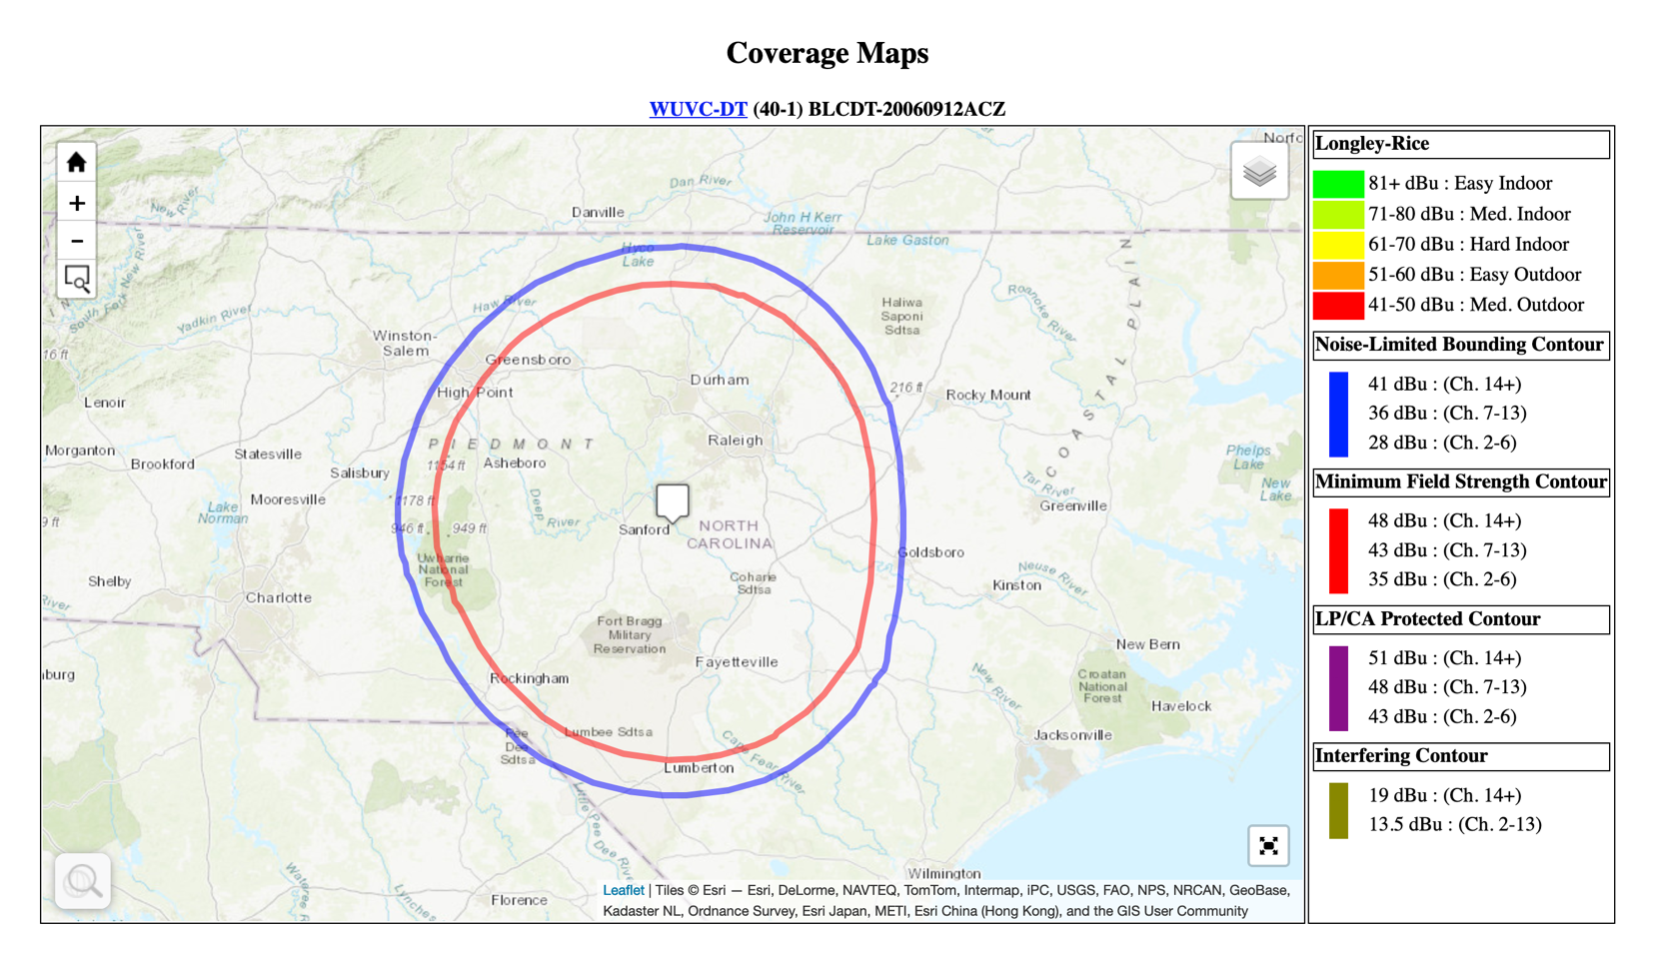
\includegraphics[width=1\textwidth]{../../analysis/Output/img/ContourExample.png}\\
\end{frame}

\begin{frame}
\frametitle{Specifications}

\textbf{Main Model:}
\[ Y_i^{} = \beta_0 + \beta \mathbb{I}[InsideContour_i] \times Distance_i + \gamma X_i + \epsilon_i \]

\textbf{Spatial Autogressive:}
\[ Y = \beta_0 + \rho W Y + \beta \mathbb{I}[InsideContour] \times Distance + \gamma X + \epsilon \]

\textbf{Spatial Error:}
\[ Y = \beta_0 + \beta \mathbb{I}[InsideContour] \times Distance + \gamma X + \epsilon \]
\[\epsilon = \lambda W \epsilon + \nu\]

where $W$ is a 4 nearest neighbor/rook spatial weights matrix

\end{frame}

\begin{frame}
\frametitle{Data - General}

\begin{itemize}
\item Instrument:
\begin{itemize}
\item Identify 100 Spanish Language TV stations across the US from TMS
\item Station contours and other station data from the FCC (use data from 2015 for consistency with outcomes)
\end{itemize}
\item Geocoding:
\begin{itemize}
\item ArcGIS: 99\%+ successfully geocoded, but data limit (schools and small number of campaign contributions)
\item US Census Geocoder: 80\% successfully geocoded (firms and campaign contributions)
\end{itemize}
\item Demographic and migration information at county level from ACS
\end{itemize}

\end{frame}

\begin{frame}
\frametitle{Selection? Migration?}
\begin{center}
        \scalebox{.5}{
	\begin{threeparttable}
			\begin{tabular}{lcccccccccc}
				\hline\hline\addlinespace
				& \multicolumn{3}{c}{IHS(\# Hispanic Migrants)} \\
				\cline{2-4} 
				Panel A: Origin County Inside Contour&  (1) & (2) & (3) \\
                                \hline\addlinespace
Dummy: Destination Outside TV Contour & $-$0.387$^{***}$ & $-$0.286$^{***}$ & $-$0.280$^{***}$ \\ 
  & (0.048) & (0.044) & (0.044) \\ 
 TV Dummy $\times$ Distance to Origin & $-$0.003$^{**}$ & $-$0.004$^{***}$ & $-$0.004$^{***}$ \\ 
  & (0.001) & (0.001) & (0.001) \\ 
 TV Dummy $\times$ Distance to Destination & 0.001 & $-$0.002$^{*}$ & $-$0.002 \\ 
  & (0.001) & (0.001) & (0.001) \\ 
 Distance from Contour to Origin (KM) & 0.001 & 0.003$^{*}$ & 0.003 \\ 
  & (0.002) & (0.002) & (0.002) \\ 
 Distance from Contour to Destination (KM) & $-$0.001 & 0.002 & 0.002 \\ 
  & (0.001) & (0.001) & (0.001) \\ 
Observations & 8,479 & 8,479 & 8,479 \\ 
\hline\addlinespace
Panel B: Origin County Outside Contour & & & \\ 
\hline\addlinespace
 Dummy: Destination Inside TV Contour & $-$0.078 & $-$0.123 & $-$0.120 \\ 
  & (0.108) & (0.096) & (0.096) \\ 
 TV Dummy $\times$ Distance to Origin & $-$0.003$^{*}$ & $-$0.004$^{***}$ & $-$0.004$^{***}$ \\ 
  & (0.002) & (0.001) & (0.001) \\ 
 TV Dummy $\times$ Distance to Destination & $-$0.004$^{***}$ & $-$0.002 & $-$0.002 \\ 
  & (0.001) & (0.001) & (0.001) \\ 
 Distance from Contour to Origin (KM) & $-$0.0003 & 0.001 & 0.001 \\ 
  & (0.001) & (0.001) & (0.001) \\ 
 Distance from Contour to Destination (KM) & $-$0.001$^{***}$ & $-$0.001$^{***}$ & $-$0.001$^{***}$ \\ 
  & (0.0002) & (0.0003) & (0.0003) \\ 
Observations & 4,062 & 4,062 & 4,062 \\         
\hline\addlinespace
                                Log(Population) & Yes & Yes  & Yes\\
                                County \% Hispanic & No & Yes & Yes\\
                                Log(Income) & No & No & Yes\\
				\addlinespace\hline\hline
			\end{tabular}
			\begin{tablenotes}[flushleft]
				\item \textit{Notes:} County-county data with origin F.E. 
			\end{tablenotes}
		\end{threeparttable}

        }
\end{center}
\end{frame}

\begin{frame}
\frametitle{Firms}

\begin{itemize}
\item Data from Florida's Division of Corporations
\begin{itemize}
\item Why Florida? 23\% Hispanic (8\% US total), 11 SLTV stations (11\% total) and open data
\item 146,032 firms successfully geocoded
\item Aggregate data into $2\times 2$ KM$^2$ squares
\end{itemize}
\item Firm Owner Name Classification
\begin{itemize}
\item `ethnicolr' --- a LSTM model trained with TensorFlow on Florida voter registration data
\item Validation $>85\%$ accurate, $23.5\%$ firm owners are Hispanic
\end{itemize}
\item Firm Name Classification
\begin{itemize}
\item Keyword matching on (1) references to Latin American countries, (2) top 50 most common Spanish words not in English, and optionally (3) references to common Hispanic foods
\item 1\% (1.1\% with food) of firms match this criteria
\end{itemize}
\end{itemize}
\end{frame}



\begin{frame}
\frametitle{Firms - Summary Statistics}
\begin{center}
\scalebox{.75}{
               \begin{threeparttable}
			\begin{tabular}{l@{\extracolsep{4pt}}cccc}
				\hline\hline\addlinespace
				& \textit{All} &  \textit{No TV} & \textit{TV} \\
				\cline{2-4} \addlinespace
				& (1) & (2) & (3) \\
				\hline\addlinespace Panel A: Firms & \multicolumn{3}{c}{} \\
				\hline\addlinespace
				IHS(Hispanic Owned Firms) & 0.992 & 0.671 & 1.225 \\
				& (1.694) & (1.308) & (1.892) \\
				Hispanic Named Firms & 0.027  & 0.006 & 0.042 \\
				& (0.161) & (0.080) & (0.200) \\
				Log Income & 9.498 & 9.463 & 9.523 \\
				& (0.241) & (0.284) & (0.201) \\
				Log Population & 11.954 & 11.206 & 12.497 \\
				& (1.398) & (1.253) & (1.239) \\
				Fraction County Hispanic & 0.086 & 0.063 & 0.103 \\
				& (0.105) & (0.061) & (0.125) \\
				Observations & 23,823 & 10,023 & 13,830\\
				\hline\addlinespace
				 \hline\addlinespace
			\end{tabular}
			\begin{tablenotes}[flushleft]
				\item \textit{Notes:} The table presents means (and standard deviations). No control is significantly different across the coverage contour at the $\alpha = .1$ level.
			\end{tablenotes}
		\end{threeparttable}
        }
\end{center}
\end{frame}

\begin{frame}
\frametitle{Effect of SLTV on Hispanic Firm Ownership}
\begin{center}
\scalebox{.75}{
		\begin{threeparttable}
			\begin{tabular}{lcccccccccc}
				\hline\hline\addlinespace
				 & \multicolumn{4}{c}{\textit{IHS(\# Hispanic Owned Businesses)}}\\
				&  (1) & (2) & (3) & (4) \\
                                \hline\addlinespace
 TV Dummy & 0.261$^{***}$ & 0.122$^{***}$ & 0.112$^{***}$ & 0.132$^{***}$ \\ 
  & (0.014) & (0.014) & (0.014) & (0.015) \\ 
 TV Dummy $\times$ Distance to Boundary & 0.010$^{***}$ & 0.007$^{***}$ & 0.007$^{***}$ & 0.007$^{***}$ \\ 
  & (0.001) & (0.001) & (0.001) & (0.001) \\ 
 Distance to Boundary (meters) & 0.006$^{***}$ & 0.009$^{***}$ & 0.010$^{***}$ & 0.011$^{***}$ \\ 
  & (0.001) & (0.001) & (0.001) & (0.001) \\ 
 Log(Population) &  & 0.412$^{***}$ & 0.388$^{***}$ & 0.342$^{***}$ \\ 
  &  & (0.011) & (0.012) & (0.014) \\ 
 County \% Hispanic &  &  & 1.261$^{***}$ & 1.414$^{***}$ \\ 
  &  &  & (0.133) & (0.136) \\ 
 Log(Income) &  &  &  & 0.391$^{***}$ \\ 
  &  &  &  & (0.070) \\ 
Observations & 23,853 & 23,853 & 23,853 & 23,853 \\ 
				\addlinespace\hline\hline
			\end{tabular}
			\begin{tablenotes}[flushleft]
				\item \textit{Notes:} 
			\end{tablenotes}
		\end{threeparttable}
        }
\end{center}
\end{frame}

\begin{frame}
\frametitle{Effect of SLTV on Hispanic Firm Ownership - Spatial Robustness}
\begin{center}
\scalebox{.8}{
\begin{threeparttable}
			\begin{tabular}{lcccccccccc}
				\hline\hline\addlinespace
				 & \multicolumn{3}{c}{\textit{IHS(\# Hispanic Owned Firms)}}\\
				&  (1) & (2) & (3) \\
                                \hline\addlinespace
 TV Dummy & 0.122$^{***}$ & 0.022$^{***}$ & 0.126$^{***}$ \\ 
  & (0.014) & (0.006) & (0.036) \\ 
\hline\hline\addlinespace
Observations & 23,853 & 23,853 & 23,853 \\ 
Log Likelihood &  & $-$38,404 & $-$38,440 \\ 
$\sigma^{2}$ &  & 1.168 & 1.170 \\ 
Akaike Inf. Crit. &  & 76,821 & 76,894 \\ 
Wald Test (df = 1) &  & 65,139$^{***}$ & 63,913$^{***}$ \\ 
LR Test (df = 1) &  & 24,759$^{***}$ & 24,687$^{***}$ \\ 
\hline \addlinespace
                                County Controls & Yes & Yes  & Yes \\
                                Model & OLS & SAR Lag & SAR Error \\
				\addlinespace\hline\hline
			\end{tabular}
			\begin{tablenotes}[flushleft]
				\item \textit{Notes:} 
			\end{tablenotes}
		\end{threeparttable}
        }
\end{center}
\end{frame}

\begin{frame}
\frametitle{Effect of SLTV on Hispanic Firm Names}
\begin{center}
\scalebox{.85}{
\begin{threeparttable}
			\begin{tabular}{lcccccccccc}
				\hline\hline\addlinespace
				 & \multicolumn{3}{c}{\textit{IHS(\# Hispanic Owned Firms)}}\\
				&  (1) & (2) & (3) \\
                                \hline\addlinespace
 TV Dummy & 0.122$^{***}$ & 0.022$^{***}$ & 0.126$^{***}$ \\ 
  & (0.014) & (0.006) & (0.036) \\ 
\hline\hline\addlinespace
Observations & 23,853 & 23,853 & 23,853 \\ 
Log Likelihood &  & $-$38,404 & $-$38,440 \\ 
$\sigma^{2}$ &  & 1.168 & 1.170 \\ 
Akaike Inf. Crit. &  & 76,821 & 76,894 \\ 
Wald Test (df = 1) &  & 65,139$^{***}$ & 63,913$^{***}$ \\ 
LR Test (df = 1) &  & 24,759$^{***}$ & 24,687$^{***}$ \\ 
\hline \addlinespace
                                County Controls & Yes & Yes  & Yes \\
                                Model & OLS & SAR Lag & SAR Error \\
				\addlinespace\hline\hline
			\end{tabular}
			\begin{tablenotes}[flushleft]
				\item \textit{Notes:} 
			\end{tablenotes}
		\end{threeparttable}
        }
\end{center}
\end{frame}

\begin{frame}
\frametitle{Effect of SLTV on Hispanic Firm Names}
\begin{center}
\scalebox{.65}{
\begin{threeparttable}
			\begin{tabular}{lcccccccccc}
				\hline\hline\addlinespace
				 & \multicolumn{6}{c}{\textit{Hispanic Named Business Dummy}}\\
				&  (1) & (2) & (3) & (4) & (5) & (6) \\
                                \hline\addlinespace
 TV Dummy & 0.839$^{***}$ & 0.638$^{***}$ & 0.637$^{***}$ & 0.769$^{***}$ & 0.849$^{***}$ & 0.775$^{***}$ \\ 
  & (0.052) & (0.066) & (0.066) & (0.071) & (0.077) & (0.071) \\ 
 TV Dummy $\times$ Distance to Boundary & 0.008$^{***}$ & 0.002 & 0.002 & 0.0002 & $-$0.0002 & 0.0002 \\ 
  & (0.002) & (0.002) & (0.002) & (0.002) & (0.002) & (0.002) \\ 
 Distance to Boundary (meters) & 0.010$^{**}$ & 0.021$^{***}$ & 0.021$^{***}$ & 0.031$^{***}$ & 0.035$^{***}$ & 0.031$^{***}$ \\ 
  & (0.004) & (0.004) & (0.005) & (0.005) & (0.005) & (0.005) \\ 
 Log(Population) &  & 0.957$^{***}$ & 0.979$^{***}$ & 0.702$^{***}$ & 0.761$^{***}$ & 0.701$^{***}$ \\ 
  &  & (0.052) & (0.070) & (0.074) & (0.081) & (0.074) \\ 
 County \% Hispanic &  &  & $-$0.151 & 1.428$^{***}$ & 1.514$^{***}$ & 1.434$^{***}$ \\ 
  &  &  & (0.312) & (0.367) & (0.388) & (0.368) \\ 
 Log(Income) &  &  &  & 2.350$^{***}$ & 2.534$^{***}$ & 2.356$^{***}$ \\ 
  &  &  &  & (0.319) & (0.344) & (0.320) \\ 
Observations & 23,853 & 23,853 & 23,853 & 23,853 & 23,853 & 23,853 \\ 
				\hline\hline\addlinespace
				Only Hispanic Owners & No & No & No & No & Yes & No \\
				Only Non-Hispanic Owners & No & No & No & No & No & Yes \\
				\addlinespace\hline\hline
			\end{tabular}
			\begin{tablenotes}[flushleft]
				\item \textit{Notes:} Logit regression
			\end{tablenotes}
		\end{threeparttable}

        }
\end{center}
\end{frame}

\begin{frame}
\frametitle{Effect of SLTV on Hispanic Firm Names - Robustness}
\label{firm_robust}
\begin{center}
\scalebox{.75}{
		\begin{threeparttable}
			\begin{tabular}{lcccccccccc}
				\hline\hline\addlinespace
				 & \multicolumn{4}{c}{\textit{Hispanic Owned \& Named Business Dummy}}\\
				&  (1) & (2) & (3) & (4) \\
                                \hline\addlinespace
 TV Dummy & 0.849$^{***}$ & 1.071$^{***}$ & 0.305$^{***}$ & .8677$^{***}$ \\ 
  & (0.077) & (0.115) & (0.078) & (0.079)  \\ 
 TV Dummy $\times$ Distance to Boundary  & $-$0.0002 & $-$0.008 & $-$0.003 & $-$0.001 \\ 
  & (0.002) & (0.007) & (0.002) & (0.002)  \\ 
 Distance to Boundary (meters) & 0.035$^{***}$ & 0.123$^{***}$ & 0.013$^{***}$ & 0.036$^{***}$ \\ 
  & (0.005) & (0.021) & (0.005) & (0.005)  \\ 
 Total Businesses &  &  & 0.023$^{***}$ &  \\ 
  &  &  & (0.001) &   \\ 
\hline \\[-1.8ex] 
Observations & 23,853 & 23,853 & 23,853 & 23,853  \\
 				\hline\hline\addlinespace
County Controls & Yes & Yes & Yes & Yes  \\
Distance$^2$ & No & Yes & No & No  \\
No Food Names & No & No & No & Yes \\
				\addlinespace\hline\hline
			\end{tabular}
			\begin{tablenotes}[flushleft]
				\item \textit{Notes:} Logit regressions
			\end{tablenotes}
		\end{threeparttable}

        }
\end{center}
 \hyperlink{firm_dist}{\beamergotobutton{Robustness: Vary Boundary Cut-Off and Grid Size}}
\end{frame}

\begin{frame}
\frametitle{Firms: Closing Thoughts}
\begin{itemize}
\item Existing literature finds entrepreneurship difficult to foster {\footnotesize (Karlan \& Valdiva (2011); Gine \& Mansuri 2014)}. We find signs of this, but no data on firm size. \\
\item Business naming demonstrates an appeal to identity (disproportionate increase) \\
\item Definite demand effect, supply side less clear
\end{itemize}
\end{frame}


%%%%%% SCHOOLS %%%%%%
\begin{frame}
\frametitle{Schools}
\begin{itemize}
\item Data from Department of Education's Civil Rights Data Collection in 2015:
\begin{itemize}
\item 48,000 public schools in sample (unit of observation)
\item (Almost) all variables split by ethnicity
\end{itemize}
\item Educational Attainment
\begin{itemize}
\item Gifted Program Enrolment
\item AP Program Enrolment and Exam Passes
\item Limited English Proficiency (LEP)
\end{itemize}
\item Discipline
\begin{itemize}
\item Out of School Suspensions
\item Chronic Absentees
\item Ethnicity-Based Bullying/Harassment
\end{itemize}
\end{itemize}
\end{frame}

\begin{frame}
\frametitle{Schools - Summary Statistics - Outcomes}
\begin{center}
\scalebox{.75}{
               \begin{threeparttable}
			\begin{tabular}{l@{\extracolsep{4pt}}cccc}
				\hline\hline\addlinespace
				& \textit{All} &  \textit{No TV} & \textit{TV} \\
				\cline{2-4} \addlinespace
				& (1) & (2) & (3) \\
				Panel A: Schools & \multicolumn{3}{c}{} \\
				\hline\addlinespace
				IHS(Hispanic Gifted Students) & 1.988 & 1.262 & 2.380 \\
				& (1.552) & (1.238) & (1.563) \\
				IHS(Hispanic AP Enrolment) & 3.192 & 2.091 & 3.778 \\
				& (1.937) & (0.646) & (0.918) \\
				IHS(Hispanic AP Passes) & 4.087 & 3.497 & 4.181 \\
				 & (0.917) & (0.646) & (0.918) \\
				 IHS(Hispanic Suspensions) & 0.957 & 0.676 & 1.102 \\
				 & (1.273) & (1.044) & (1.353) \\
				 IHS(Hispanic Absentees) & 2.655 & 1.881 & 3.054 \\
				 & (1.765) & (1.536) & (1.742) \\
				 IHS(Hispanic Limited English Proficiency) & 2.915 & 2.113 & 3.331 \\
				 & (2.040) & (1.820) & (2.024) \\
				 IHS(Hispanic Harassment) & 0.045 & 0.027 & 0.055 \\
				 & (0.273) & (0.211) & (0.299) \\
				 Observations & 41,502 & 11,252 & 30,250 \\
				\hline\addlinespace
				 \hline\addlinespace
			\end{tabular}
			\begin{tablenotes}[flushleft]
				\item \textit{Notes:} The table presents means (and standard deviations). 
			\end{tablenotes}
		\end{threeparttable}
        }
\end{center}
\end{frame}

\begin{frame}
\frametitle{Schools - Summary Statistics - Controls}
\begin{center}
\scalebox{.75}{
               \begin{threeparttable}
			\begin{tabular}{l@{\extracolsep{4pt}}cccc}
				\hline\hline\addlinespace
				& \textit{All} &  \textit{No TV} & \textit{TV} \\
				\cline{2-4} \addlinespace
				& (1) & (2) & (3) \\
				Panel A: Schools & \multicolumn{3}{c}{} \\
				\hline\addlinespace
				 Log Income & 9.547 & 9.430 & 9.608 \\
				 & (0.303) & (0.200) & (0.328) \\
				 Log Population & 12.484 & 11.559 & 12.964 \\
				 & (1.576) & (1.471) & (1.405) \\
				 Fraction County Hispanic & 0.107 & 0.037 & 0.143 \\
				 & (0.160) & (0.079) & (0.179) \\
				 \# School Teachers & 39.591 & 32.684 & 43.169 \\
				 & (30.764) & (24.090) & (33.146)\\
				 \# Hispanic Students & 164.343 & 68.500  & 214.011 \\
				 & (259.096) & (117.433) & (295.883) \\
				 \# Total Students & 581.524 & 478.166 & 635.086 \\
				 & (482.595) & (383.924) & (518.467) \\
				 Observations & 41,502 & 11,252 & 30,250 \\
				\hline\addlinespace
				 \hline\addlinespace
			\end{tabular}
			\begin{tablenotes}[flushleft]
				\item \textit{Notes:} The table presents means (and standard deviations). No control is significantly different across the coverage contour at the $\alpha = .1$ level.
			\end{tablenotes}
		\end{threeparttable}
        }
\end{center}
\end{frame}

\begin{frame}
\frametitle{Effect of SLTV on Hispanic Educational Attainment}
\begin{center}
\scalebox{.8}{
	\begin{threeparttable}
			\begin{tabular}{lcccccccccc}
				\hline\hline\addlinespace
				Panel A: IHS(\# Hispanic Gifted Students) &  (1) & (2) & (3) \\
                                \hline\addlinespace
 TV Dummy & 0.016$^{***}$ & 0.015$^{**}$ & 0.013$^{**}$ \\ 
  & (0.006) & (0.006) & (0.006) \\ 
Observations & 26,065 & 26,065 & 26,065 \\           
\hline\hline\addlinespace
Panel B: IHS(\# Hispanic Students Taking AP) & & & \\ 
\hline\addlinespace
 TV Dummy & 0.072$^{***}$ & 0.051$^{***}$ & 0.047$^{***}$ \\ 
  & (0.016) & (0.015) & (0.015) \\ 
Observations & 6,089 & 6,089 & 6,089 \\     
\hline\hline\addlinespace
Panel C: IHS(\# Hispanic Students Passing AP) &&& \\ 
\hline\addlinespace
 TV Dummy & 0.034$^{**}$ & 0.042$^{***}$ & 0.039$^{***}$ \\ 
  & (0.014) & (0.013) & (0.013) \\ 
Observations & 2,205 & 2,205 & 2,205 \\                 
\hline\hline\addlinespace
                                County Controls & Yes & Yes  & Yes\\
                                School Size Controls & No & Yes & Yes\\
                                School Type Controls & No & No & Yes \\
				\addlinespace\hline\hline
			\end{tabular}
			\begin{tablenotes}[flushleft]
				\item \textit{Notes:} 
			\end{tablenotes}
		\end{threeparttable}
        }
\end{center}
\end{frame}

\begin{frame}
\frametitle{Effect of SLTV on Hispanic School Discipline}
\begin{center}
\scalebox{.8}{
		\begin{threeparttable}
			\begin{tabular}{lcccccccccc}
				\hline\hline\addlinespace
				Panel A: IHS(Out of School Suspensions) &  (1) & (2) & (3) \\
                                \hline\addlinespace
 TV Dummy & $-$0.011$^{**}$ & $-$0.018$^{***}$ & $-$0.016$^{***}$ \\ 
  & (0.005) & (0.005) & (0.005) \\ 
Observations & 40,864 & 40,864 & 40,864 \\        
\hline\hline\addlinespace
Panel B: IHS(Students Chronically Absent) & & & \\ 
\hline\addlinespace
 TV Dummy & $-$0.067$^{***}$ & $-$0.073$^{***}$ & $-$0.074$^{***}$ \\ 
  & (0.006) & (0.006) & (0.006) \\ 
  Observations & 40,869 & 40,869 & 40,869 \\ 
\hline\hline\addlinespace
                                County Controls & Yes & Yes  & Yes\\
                                School Size Controls & No & Yes & Yes\\
                                School Type Controls & No & No & Yes \\
				\addlinespace\hline\hline
			\end{tabular}
			\begin{tablenotes}[flushleft]
				\item \textit{Notes:} 
			\end{tablenotes}
		\end{threeparttable}
        }
\end{center}
\end{frame}

\begin{frame}
\frametitle{Effect of SLTV on Hispanic School Identity}
\begin{center}
\scalebox{.8}{
\begin{threeparttable}
			\begin{tabular}{lcccccccccc}
				\hline\hline\addlinespace
				Panel A: IHS(Limited English Proficiency) &  (1) & (2) & (3) \\
                                \hline\addlinespace
 TV Dummy & 0.040$^{***}$ & 0.039$^{***}$ & 0.031$^{***}$ \\ 
  & (0.007) & (0.007) & (0.007) \\ 
Observations & 40,864 & 40,864 & 40,864 \\        
\hline\hline\addlinespace
Panel B: IHS(Victims of Harassment) & & & \\ 
\hline\addlinespace
TV Dummy & 0.003$^{**}$ & 0.002$^{*}$ & 0.002$^{*}$ \\ 
  & (0.001) & (0.001) & (0.001) \\ 
  Observations & 40,811 & 40,811 & 40,811 \\ 
\hline\hline\addlinespace
                                County Controls & Yes & Yes  & Yes\\
                                School Size Controls & No & Yes & Yes\\
                                School Type Controls & No & No & Yes \\
				\addlinespace\hline\hline
			\end{tabular}
			\begin{tablenotes}[flushleft]
				\item \textit{Notes:} 
			\end{tablenotes}
		\end{threeparttable}
        }
\end{center}
\end{frame}

\begin{frame}
\frametitle{Schools: Closing Thoughts}
\label{schl_close}
\begin{itemize}
\item  Robustness \hyperlink{schl_robust}{\beamergotobutton{Robustness}}  \hyperlink{schl_spatial}{\beamergotobutton{Spatial}}
\item Broadly prosocial main effects support {\footnotesize(Gentzkow \& Shapiro 2008)} against mainstream findings {\footnotesize (Gentile 2004; Zavodny 2006)}
\item Contrasting effect within identity --- consistent story of identity being strengthened
\end{itemize}
\end{frame}

\begin{frame}
\frametitle{Campaign Contributions}
\begin{itemize}
\item Data from the Federal Election Commission on 2016 Presidential Election:
\begin{itemize}
\item 651,404 addresses donated to Trump, 41,080 addresses donated to Clinton
\item Aggregate data into $2 \times 2$ KM$^2$ squares
\end{itemize}
\item Donor Names also classified with `ethnicolr'
\item Data censored for contributions beneath $\$200$
\end{itemize}
\end{frame}

\begin{frame}
\frametitle{Campaign Contributions - Summary Statistics}
\begin{center}
\scalebox{.75}{
               \begin{threeparttable}
			\begin{tabular}{l@{\extracolsep{4pt}}cccc}
				\hline\hline\addlinespace
				& \textit{All} &  \textit{No TV} & \textit{TV} \\
				\cline{2-4} \addlinespace
				& (1) & (2) & (3) \\
				Panel A: Campaign Contributions & \multicolumn{3}{c}{} \\
				\hline\addlinespace
				Hispanic Trump Donations & 0.080 & 0.032 & 0.175 \\
				& (1.165) & (0.047) & (1.900) \\
				Hispanic Clinton Donations & 0.049 & 1.407 & 1.187 \\
				& (3.014) & (1.476) & (4.773)\\
				Log Income & 9.279 & 9.253 & 9.329 \\
				& (0.270) & (0.232) & (0.327) \\
				Log Population & 10.830 & 10.084 & 10.969 \\
				& (1.514) & (1.372) & (1.607) \\
				Fraction County Hispanic & 0.148 & 0.134 & 0.176 \\
				& (0.214) & (0.200) & (0.236) \\
				Observations & 619,011 & 411,673 & 207,338 \\
				\hline\addlinespace
				 \hline\addlinespace
			\end{tabular}
			\begin{tablenotes}[flushleft]
				\item \textit{Notes:} The table presents means (and standard deviations). No control is significantly different across the coverage contour at the $\alpha = .1$ level.
			\end{tablenotes}
		\end{threeparttable}
        }
\end{center}
\end{frame}

\begin{frame}
\frametitle{Effect of SLTV on Campaign Contributions}
\begin{center}
\scalebox{.7}{
		\begin{threeparttable}
			\begin{tabular}{lcccccccccc}
				\hline\hline\addlinespace
				& \multicolumn{4}{c}{\# Hispanic Campaign Contributions} \\
				\cline{2-5} 
				Panel A: Contributions to Trump &  (1) & (2) & (3) & (4) \\
                                \hline\addlinespace
 TV Dummy & 0.019$^{***}$ & 0.010$^{***}$ & 0.007$^{***}$ & 0.005$^{***}$ \\ 
  & (0.001) & (0.001) & (0.001) & (0.001) \\ 
 TV Dummy $\times$ Distance to Boundary  & 0.002$^{***}$ & 0.001$^{***}$ & 0.001$^{***}$ & 0.001$^{***}$ \\ 
  & (0.0001) & (0.0001) & (0.0001) & (0.0001) \\ 
 Distance to Boundary (KM) & 0.0001 & 0.0003$^{***}$ & 0.0003$^{***}$ & 0.0004$^{***}$ \\ 
  & (0.0001) & (0.0001) & (0.0001) & (0.0001) \\ 
Observations & 619,011 & 619,011 & 619,011 & 619,011 \\ 
\hline\addlinespace
Panel B: Contributions to Clinton & & & \\ 
\hline\addlinespace
 TV Dummy & $-$0.008$^{**}$ & $-$0.014$^{***}$ & $-$0.019$^{***}$ & $-$0.020$^{***}$ \\ 
  & (0.004) & (0.004) & (0.004) & (0.004) \\ 
 TV Dummy $\times$ Distance to Boundary  & 0.003$^{***}$ & 0.002$^{***}$ & 0.002$^{***}$ & 0.002$^{***}$ \\ 
  & (0.0001) & (0.0001) & (0.0001) & (0.0001) \\ 
 Distance to Boundary (KM) & 0.0002 & 0.0004$^{**}$ & 0.0004$^{***}$ & 0.0004$^{***}$ \\ 
  & (0.0001) & (0.0001) & (0.0001) & (0.0001) \\ 
Observations & 619,011 & 619,011 & 619,011 & 619,011 \\ 
				\addlinespace\hline\hline
			\end{tabular}
			\begin{tablenotes}[flushleft]
				\item \textit{Notes:} 
			\end{tablenotes}
		\end{threeparttable}
		        }
\end{center}
\end{frame}

\begin{frame}
\frametitle{Campaign Contributions: Closing Thoughts}
\begin{itemize}
\item Mostly suggestive, but potentially reconciles differing results found in literature {\footnotesize(Waldfogel \& al. 2009; Velez \& Newman (2019))}
\item Why would SLTV increase contributions to Trump?
\begin{itemize}
\item Content from Latin America --- recent populist governments or social conservativeness
\item Still a Hispanic base that supports Trump (immigration etc.)
\end{itemize}
\end{itemize}
\end{frame}

\begin{frame}
\frametitle{Conclusion}
\begin{itemize}
\item SLTV creates a variety of effects: more firms, fewer disciplinary issues, political campaign contributions
\item Underlying theme of strengthened identity
\item Lots of space for future work
\end{itemize}
\end{frame}

		
\begin{frame}
\Large \centering \textcolor{darkblue}{Thank You!}
\end{frame}

%%%%%%% APPENDIX %%%%%%%%%%

\begin{frame}
\frametitle{Effect of SLTV on Hispanic Firm Names - Different Boundary/Grid Sizes}
\label{firm_dist}
\begin{center}
\scalebox{.6}{
		\begin{threeparttable}
			\begin{tabular}{lcccccccccc}
				\hline\hline\addlinespace
				 & \multicolumn{5}{c}{\textit{Hispanic Owned \& Named Business Dummy}}\\
				&  (1) & (2) & (3) & (4) & (5) \\
                                \hline\addlinespace
 TV Dummy & 0.849$^{***}$  & 0.927$^{***}$ & 0.596$^{***}$ & 0.624$^{***}$ & 1.144$^{***}$ \\ 
  & (0.077)  & (0.098) & (0.118) & (0.078) & (0.076) \\ 
 TV Dummy $\times$ Distance to Boundary  & $-$0.0002 & $-$0.002 & 0.042$^{***}$ & 0.001 & $-$0.001 \\ 
  & (0.002) & (0.004) & (0.010) & (0.002) & (0.002)   \\ 
 Distance to Boundary (meters) & 0.035$^{***}$ & 0.049$^{***}$ & $-$0.097$^{***}$ & 0.026$^{***}$ & 0.042$^{***}$ \\ 
  & (0.005) & (0.012) & (0.035) & (0.005) & (0.006) \\ 
\hline \\[-1.8ex] 
Observations & 23,853& 20,404 & 14,386 & 10,598 & 95,373 \\ 				
 				\hline\hline\addlinespace
County Controls & Yes & Yes & Yes & Yes  & Yes \\
Distance Cutoff (KM) & 100 & 50 &25 & 100 &100 \\
Grid Size (KM$^2$) & 4 & 4 & 4 & 9 & 1\\ 
				\addlinespace\hline\hline
			\end{tabular}
			\begin{tablenotes}[flushleft]
				\item \textit{Notes:} Logit regressions
			\end{tablenotes}
		\end{threeparttable}
        }
\end{center}
 \hyperlink{firm_robust}{\beamergotobutton{Back}}
\end{frame}

\begin{frame}
\frametitle{Effect of SLTV on Hispanic Educational Attainment - Robustness}
\label{schl_robust}
\begin{center}
\scalebox{.6}{
		\begin{threeparttable}
			\begin{tabular}{lcccccccccc}
				\hline\hline\addlinespace
				 & \multicolumn{6}{c}{\textit{IHS(\# Hispanic Students Passing AP)}}\\
				&  (1) & (2) & (3) & (4) & (5) & (6) \\
                                \hline\addlinespace
 TV Dummy & 0.039$^{***}$ & 0.049$^{***}$ & 0.044$^{***}$ & 0.044$^{***}$ & 0.036$^{***}$ & 0.032$^{*}$ \\ 
  & (0.013) & (0.017) & (0.016) & (0.017) & (0.013) & (0.018) \\ 
 TV Dummy $\times$ Distance to Boundary & 0.0003 & 0.0001 & 0.001 & 0.001$^{*}$ & 0.0001 & 0.001 \\ 
  & (0.0002) & (0.001) & (0.001) & (0.0004) & (0.0004) & (0.001) \\ 
 Distance to Boundary (meters) & 0.001 & 0.012$^{***}$ & 0.006$^{***}$ & 0.006$^{***}$ & 0.003$^{**}$ & 0.001 \\ 
  & (0.001) & (0.003) & (0.002) & (0.002) & (0.002) & (0.004) \\ 
 Total APs Passed &  &  &  &  & 0.003$^{***}$ &  \\ 
  &  &  &  &  & (0.0001) &  \\ 
Observations & 2,205 & 2,205 & 1,525 & 1,525 & 1,525 & 1,095 \\ 
\hline\hline\addlinespace
                                County/School Controls & Yes & Yes  & Yes & Yes & Yes & Yes\\
                                Distance Cutoff (KM) & 100 & 100 & 50 & 50 & 50 & 33 $\frac{1}{3}$ \\
                                Distance$^{2}$ Interaction & No & Yes & No & No & No & No \\
                                County F.E. & No & No & No & Yes & No & No  \\
				\addlinespace\hline\hline
			\end{tabular}
			\begin{tablenotes}[flushleft]
				\item \textit{Notes:} 
			\end{tablenotes}
		\end{threeparttable}
        }
\end{center}
 \hyperlink{schl_close}{\beamergotobutton{Back}}
\end{frame}

\begin{frame}
\frametitle{Effect of SLTV on Hispanic Identity - Spatial Robustness}
\label{schl_spatial}
\begin{center}
\scalebox{.8}{
		\begin{threeparttable}
			\begin{tabular}{lcccccccccc}
				\hline\hline\addlinespace
				 & \multicolumn{3}{c}{\textit{IHS(\# Hispanic Victims of Harassment)}}\\
				&  (1) & (2) & (3) \\
                                \hline\addlinespace
 TV Dummy & 0.003$^{**}$ & 0.002$^{***}$ & 0.003$^{*}$ \\ 
  & (0.001) & (0.001) & (0.002) \\ 
 TV Dummy $\times$ Distance to Boundary & $-$0.0001$^{**}$ & $-$0.0001$^{***}$ & $-$0.0001$^{**}$ \\ 
  & (0.00002) & (0.00001) & (0.00003) \\ 
\hline\hline\addlinespace
Observations & 40,811 & 40,811 & 40,811 \\ 
Log Likelihood &  & $-$4,304.916 & $-$4,299.820 \\ 
$\sigma^{2}$ &  & 0.072 & 0.072 \\ 
Akaike Inf. Crit. &  & 8,629.833 & 8,619.640 \\ 
Wald Test (df = 1) &  & 686.149$^{***}$ & 686.981$^{***}$ \\ 
LR Test (df = 1) &  & 657.312$^{***}$ & 667.505$^{***}$ \\ 
\hline \addlinespace
                                County/School Controls & Yes & Yes  & Yes \\
                                Model & OLS & SAR Lag & SAR Error \\
				\addlinespace\hline\hline
			\end{tabular}
			\begin{tablenotes}[flushleft]
				\item \textit{Notes:} 
			\end{tablenotes}
		\end{threeparttable}
        }
\end{center}
 \hyperlink{schl_close}{\beamergotobutton{Back}}
\end{frame}



\end{document}


























